%%%%%%%%%% Commands --

%% General commands
\newcommand{\todo}[1]{\emph{\textcolor{red}{TODO: #1}}}
\newcommand{\note}[1]{\emph{\textcolor{blue}{NOTE: #1}}}
\newcommand{\panic}[1]{\textbf{\textcolor{red}{(#1)}}}

\renewcommand{\subsectionautorefname}{section}
\renewcommand{\subsubsectionautorefname}{section}

\newcommand{\ie}{i.e.,}
\newcommand{\eg}{e.g.,}
\newcommand{\aka}{a.k.a.}

\newcommand{\tuple}[1]{\langle #1 \rangle}
\renewcommand\qedsymbol{$\blacksquare$}

%% Hemiola

\newcommand{\hemiola}{Hemiola}

\newcommand{\listof}[1]{\ensuremath{\mathbf{#1}}}
\newcommand{\listtof}[1]{\ensuremath{\overrightarrow{#1}}}
\newcommand{\listnil}{\ensuremath{\lbrack\rbrack}}
\newcommand{\listcons}[2]{\ensuremath{#1 : #2}}
\newcommand{\listsingle}[1]{\ensuremath{\lbrack #1 \rbrack}}
\newcommand{\listapp}[2]{\ensuremath{#1 + #2}}
\newcommand{\listsub}[2]{\ensuremath{#1 - #2}}
\newcommand{\listdisj}[2]{\ensuremath{#1 \; \# \; #2}}
\newcommand{\listconcat}[1]{\ensuremath{\widehat{#1}}}
\newcommand{\sizeof}[1]{\ensuremath{|\, #1\, |}}

\newcommand{\mapupd}[3]{\listapp{#1}{(#2, #3)}}
\newcommand{\mapupds}[2]{\listapp{#1}{#2}}
\newcommand{\mapsubs}[2]{\listsub{#1}{#2}}

\newcommand{\idxOf}[1]{\ensuremath{#1.i}}

\newcommand{\propt}{\ensuremath{\mathbb{P}}}
\newcommand{\hidt}{\ensuremath{\mathbb{I}}}
\newcommand{\hvaluet}{\ensuremath{\mathbb{V}}}
\newcommand{\hmsgt}{\ensuremath{\mathbb{M}}}
\newcommand{\hostt}{\ensuremath{\mathbb{O}}}
\newcommand{\hsyst}{\ensuremath{\mathbb{S}}}
\newcommand{\hidmt}{\ensuremath{\hidt \ast \hmsgt}}
\newcommand{\hprect}{\ensuremath{\mathcal{P}}}
\newcommand{\htrst}{\ensuremath{\mathcal{T}}}

\newcommand{\hsysIn}[1]{\ensuremath{\listof{#1_{\textrm{in}}}}}
\newcommand{\hsysRq}[1]{\ensuremath{\listof{#1_{\textrm{rq}}}}}
\newcommand{\hsysRs}[1]{\ensuremath{\listof{#1_{\textrm{rs}}}}}
\newcommand{\hsys}[4]{\ensuremath{\tuple{#1, #2, #3, #4}}}
\newcommand{\hsyss}[2]{\hsys{#1}{\hsysIn{#2}}{\hsysRq{#2}}{\hsysRs{#2}}}
\newcommand{\hsysInA}[1]{\ensuremath{#1.\hsysIn{i}}}
\newcommand{\hsysRqA}[1]{\ensuremath{#1.\hsysRq{i}}}
\newcommand{\hsysRsA}[1]{\ensuremath{#1.\hsysRs{i}}}

\newcommand{\hsysobjs}[1]{\ensuremath{#1.\listof{O}}}
\newcommand{\hobjrules}[1]{\ensuremath{#1.\listof{r}}}

\newcommand{\msgIns}[1]{\listof{#1^{\textrm{ins}}}}
\newcommand{\msgOuts}[1]{\listof{#1^{\textrm{outs}}}}
\newcommand{\midxIns}[1]{\listof{\idxOf{#1^{\textrm{ins}}}}}
\newcommand{\midxOuts}[1]{\listof{\idxOf{#1^{\textrm{outs}}}}}

\newcommand{\lblEmpty}{\ensuremath{l_\epsilon}}
\newcommand{\lblIns}[1]{\ensuremath{l_{\textrm{in}}(#1)}}
\newcommand{\lblOuts}[1]{\ensuremath{l_{\textrm{out}}(#1)}}
\newcommand{\lblInt}[4]{\ensuremath{l_{\textrm{int}}(#1, #2, #3, #4)}}

\newcommand{\hmpt}{\ensuremath{\mathcal{M}}}
\newcommand{\hsttr}{\ensuremath{\listtof{\hostt} \ast \hmpt}}
\newcommand{\hstt}{\ensuremath{\mathbb{S}}}
\newcommand{\hst}[2]{\ensuremath{\tuple{#1, #2}}}
\newcommand{\hstm}[2]{\ensuremath{\left\langle\begin{array}{l}#1,\\ #2 \end{array}\right\rangle}}
\newcommand{\sysInit}[1]{\ensuremath{#1_{\textsf{init}}}}

\newcommand{\disj}[2]{\ensuremath{#1 \; \# \; #2}}
\newcommand{\nodup}[1]{\ensuremath{\textsf{nodup}\: #1}}

\newcommand{\semstep}[4]{\ensuremath{#2 \xrightarrow[#1]{#3} #4}}
\newcommand{\semsteps}[4]{\ensuremath{#2 \xRightarrow[#1]{#3} #4}}
\newcommand{\semrch}[2]{\ensuremath{#1 \Rightarrow #2}}
\newcommand{\semleg}[2]{\ensuremath{#1 \xRightarrow{#2} \bullet}}
\newcommand{\sembeh}[2]{\ensuremath{#1 \Downarrow #2}}
\newcommand{\behOf}[1]{\ensuremath{\widetilde{#1}}}

\newcommand{\refines}[2]{\ensuremath{#1 \sqsubseteq #2}}

\newcommand{\enqMsgs}[2]{\mapupds{#1}{#2}}
\newcommand{\deqMsgs}[2]{\mapsubs{#1}{#2}}

%% Serializability

\newcommand{\atomic}[3]{\ensuremath{#1 \stackrel{#2}{\rightsquigarrow} #3}}
\newcommand{\atomicLong}[3]{\ensuremath{#1 \frac{\scriptstyle{#2}}{}\hspace{-5pt}\rightsquigarrow #3}}
\newcommand{\extatomic}[4]{\ensuremath{#1 \vdash #2 \stackrel{#3}{\rightsquigarrow}_{\textsf{ext}} #4}}
\newcommand{\extatomicLong}[4]{\ensuremath{#1 \vdash #2 \frac{\scriptstyle{#3}}{}\hspace{-5pt}\rightsquigarrow_{\textsf{ext}} #4}}
\newcommand{\trsn}[2]{\ensuremath{#1 \sswarrow #2}}

\newcommand{\extatomicshort}[2]{\ensuremath{#1 \stackrel{#2}{\rightsquigarrow}_{\textsf{ext}}}}
\newcommand{\intatomicshort}[2]{\ensuremath{#1 \stackrel{#2}{\rightsquigarrow}_{\textsf{int}}}}

\newcommand{\amsgi}[1]{\ensuremath{#1^{\textrm{init}}}}
\newcommand{\amsge}[1]{\ensuremath{#1^{\textrm{end}}}}

\newcommand{\hseq}[2]{\ensuremath{#1 \parallel #2}}
\newcommand{\hsrzl}[2]{\ensuremath{\mathit{Serializable}\ #1\ #2}}
\newcommand{\hsrz}[1]{\ensuremath{\mathit{Serializable}\ #1}}

\newcommand{\strsn}[2]{\ensuremath{#1 \sswarrow_{s} #2}}
\newcommand{\hsseq}[3]{\ensuremath{#1 \parallel_{#3} #2}}

%%%%%%%%%% Contents --

\section{Introduction}\label{sec-intro}

Cache-coherence protocols have been regarded as one of the greatest correctness challenges of the hardware world.
Industry has most commonly used testing and bounded model checking for quality assurance of cache-coherence implementations, but these techniques are not sound and sometimes miss subtle bugs~\cite{ccbug}.

Research on model checking and theorem proving has produced sound techniques, though typically with significant limitations:
either the verification is of a specific protocol, or state-space-explosion concerns limit applicability to quite small cache topologies~\cite{Komuravelli:2014,Murali:2015,Banks:2017,Oswald:2018}.
In order to overcome the latter, recent approaches~\cite{Chen:2008,Chen:2010,McMillan:2016,Opeoluwa:2016,Opeoluwa:2017,Oswald:2020} utilized the notion of \emph{modularity} and successfully built verification tools that are scalable enough to verify hierarchical cache-coherence protocols.

However, these modularity disciplines impose significant restrictions in protocol design, in order to obtain clear module boundaries among caches.
A concrete limitation of modular design and verification comes when trying to verify cache-coherence protocols that are not \emph{inclusive}.
Noninclusive caches have been in common industrial use for a decade: AMD Opteron servers are known to use exclusive caches~\cite{Irazoqui:2016}, and Intel Skylake-X processors use noninclusive\footnote{Intel uses the term ``noninclusive cache'' to say that the cache is neither inclusive nor exclusive.} caches~\cite{intel-non-inclusive,Zhao:2010,Yan:2019}.

I would like to view the verification of hierarchical cache-coherence protocols from a different perspective.
Instead of decomposing a protocol design and proof, we view a cache-coherence protocol as a \emph{global} distributed protocol and look for commonalities across well-designed protocols.
It is a good start to identify ``good-hygiene'' properties, but it is even better to formalize such properties in frameworks that guide the design of protocols.
Then we can provide nonobvious and useful reasoning principles by-construction.

Looking for another way to factor proofs, we can find a hint in terminology often employed by protocol designers and verification engineers.
These protocols are distributed message-passing systems, so we can apply traditional software terminology like \emph{transaction} to them directly, and in fact we find similar intuitions employed in practice.
In order to describe a case where the protocol deals with two different requests passing through the same cache, for instance, a designer often says ``this cache acts like a \emph{serialization point} so the two transactions can safely \emph{interleave} with each other.''
While the notions of interleaving and serialization are already pervasive, I have found no past work trying to find a minimal set of conditions that ensure transactions are always serialized, formalizing them in a reusable framework.

In this proposal, I propose a framework called \hemiola{}, embedded in the Coq proof assistant, which dramatically decreases the burden of designing and formally proving hierarchical cache-coherence protocols.
In particular, on top of the framework, hardware developers can design cache-coherence protocols without worrying about possible complex interleavings among different transactions, standing for different concurrent memory accesses.
From the verification perspective, it is established that any invariant of a protocol under serialized execution is also an invariant under the interleaved executions that are necessary for good performance.

More specifically, \hemiola{} formalizes a set of message-passing distributed protocols with tree hierarchies and particular topologies of channels between nodes, with associated locks.
These protocols are defined by associating each tree node with a set of local state-transition rules that may remove messages from incoming queues and add messages to outgoing queues.
\hemiola{} exposes a domain-specific language of protocols, such that any expressible program is guaranteed to validate a \emph{serializability} property for single memory requests.
Furthermore, the framework provides a novel invariant proof method that only requires consideration of execution histories that do not interleave memory accesses -- so that almost all formal reasoning about concurrency is confined to the framework, not proofs of individual protocols.

To demonstrate usability of the framework, I plan to provide complete correctness proofs of hierarchical, noninclusive cache-coherence protocols as case studies.
A compilation/synthesis toolchain will also be provided, which converts a cache-coherence protocol described in \hemiola{} to a corresponding hardware implementation running on FPGAs.
A so-called protocol compiler would take such a role, which employes predesigned, optimized hardware components such as caches and resource controllers.

\section{Motivation and Background}

\subsection{Challenges in designing cache-coherence protocols}
\label{sec-example}

Before proposing the \hemiola{} framework, we provide a simple yet motivating example to introduce cache-coherence protocols and typical challenges in the design and verification.
For simplicity, in this section, we will consider only \emph{a single memory location} and design a protocol only for this location.
We will see it is still nontrivial to design a correct protocol.

\tikzset{
  msi/.pic = {
    \node at (0, 0) {$P(S, v, S_{\tuple{1, 2}})$};
    \node at (-1.5, -1.5) {$C_1(S, v)$};
    \node at (1.5, -1.5) {$C_2(S, v)$};
    % between P and C_1
    \draw [<-<] (-0.6, -0.3) -- (-1.5, -1.2);
    \draw [<-<] (-0.4, -0.3) -- (-1.3, -1.2);
    \draw [>->] (-0.2, -0.3) -- (-1.1, -1.2);
    % between P and C_2
    \draw [<-<] (0.6, -0.3) -- (1.5, -1.2);
    \draw [<-<] (0.4, -0.3) -- (1.3, -1.2);
    \draw [>->] (0.2, -0.3) -- (1.1, -1.2);
    % C_1 external
    \draw [<-<] (-1.6, -1.8) -- (-1.6, -2.3);
    \draw [>->] (-1.4, -1.8) -- (-1.4, -2.3);
    % C_2 external
    \draw [<-<] (1.6, -1.8) -- (1.6, -2.3);
    \draw [>->] (1.4, -1.8) -- (1.4, -2.3);
  },
  msipc1/.pic = {
    \node at (0, 0) {$P(S, v, S_{\tuple{1, 2}})$};
    \node at (0, -1.5) {$C_1(S, v)$};
    % between P and C_1
    \draw [<-<] (-0.2, -0.3) -- (-0.2, -1.2);
    \draw [<-<] (0, -0.3) -- (0, -1.2);
    \draw [>->] (0.2, -0.3) -- (0.2, -1.2);
    % C_1 external
    \draw [<-<] (-0.1, -1.8) -- (-0.1, -2.3);
    \draw [>->] (0.1, -1.8) -- (0.1, -2.3);
  },
  msipc2/.pic = {
    \node at (0, 0) {$P(S, v, S_{\tuple{1, 2}})$};
    \node at (0, -1.5) {$C_2(I, \cdot)$};
    % between P and C_1
    \draw [<-<] (-0.4, -0.3) -- (-0.4, -1.2);
    \draw [<-<] (-0.2, -0.3) -- (-0.2, -1.2);
    \draw [>->] (0.4, -0.3) -- (0.4, -1.2);
    % C_1 external
    \draw [<-<] (-0.1, -1.8) -- (-0.1, -2.3);
    \draw [>->] (0.1, -1.8) -- (0.1, -2.3);
  },
  msipc3/.pic = {
    \node at (0, 0) {$P(I, \cdot, M_{\tuple{1}})$};
    \node at (0, -1.5) {$C_1(S, v)$};
    \node at (1.8, 0) {$C_2(I, \cdot)$};
    % between P and C_1
    \draw [<-<] (-0.2, -0.3) -- (-0.2, -1.2);
    \draw [<-<] (0, -0.3) -- (0, -1.2);
    \draw [>->] (0.2, -0.3) -- (0.2, -1.2);
    % between P and C_2
    \draw [<->] (0.9, 0) -- (1.2, 0);
    % C_1 external
    \draw [<-<] (-0.1, -1.8) -- (-0.1, -2.3);
    \draw [>->] (0.1, -1.8) -- (0.1, -2.3);
  },
  spec/.pic = {
    \node at (0, 0) {$\textrm{Spec}(v)$};
    % C_1 external
    \draw [<-<] (-0.4, -0.3) -- (-0.5, -0.8);
    \draw [>->] (-0.2, -0.3) -- (-0.3, -0.8);
    % C_2 external
    \draw [<-<] (0.4, -0.3) -- (0.5, -0.8);
    \draw [>->] (0.2, -0.3) -- (0.3, -0.8);
  }
}
\begin{figure}[h]
  \centering
  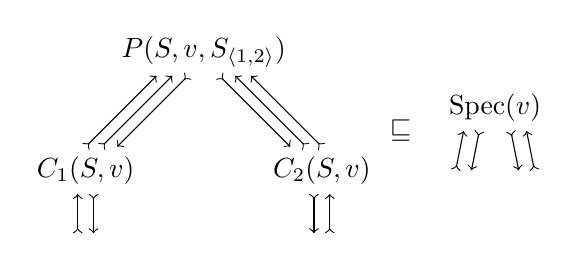
\begin{tikzpicture}
    \pic at (0, 0) {msi};
    \node at (2.5, -1) {$\sqsubseteq$};
    \pic at (3.7, -0.7) {spec};
  \end{tikzpicture}
  \caption{A simple MSI directory protocol}
  \vspace{-5pt}
  \label{fig-motive-1}
\end{figure}

The overall goal of cache coherence is, as the name suggests, to preserve coherence among multiple candidate values in a memory subsystem.
In other words, if the system is coherent, then it should behave like an ordinary memory.
\autoref{fig-motive-1} shows objects and channels for a simple directory-based MSI protocol.
Since we deal with only a single memory location, the specification (RHS of $\sqsubseteq$) is a single-value ($v$) container with atomic read and write.

Looking at the implementation (LHS of $\sqsubseteq$), there are three objects $P$, $C_1$, and $C_2$, and each of them has its own status (M, S, or I) and data ($v$).
A status of an object represents a permission on its local replica.
In this MSI protocol, an object can read/write the data with the M (``modified'') status, only read with S (``shared''), and cannot read/write with I (``invalid'').
The parent $P$ additionally has a data structure called a \emph{directory} to track the statuses of the children.
For example, a directory might be $S_{\tuple{1, 2}}$, meaning that both $C_1$ and $C_2$ have S status, in some logical snapshot of state.

Objects communicate through ordered channels (shown as $\rightarrowtail$ in the figure).
$C_1$ and $C_2$ have channels to receive and respond to external requests (from processor cores).
There are three types of channels between a parent and a child: a single channel for parent-to-child messages and two channels for child-to-parent requests and responses, respectively.
It is natural to wonder why two separate channels are required from a child to a parent; we will see the reason very soon.
Note that channels are depicted in a logical way; the actual hardware implementation may use different hardware components (\eg{} finite-capacity FIFOs or buses) that can simulate ordered channels.

\newcommand{\blackdiamond}{\raisebox{.4ex}{\ensuremath{\scriptscriptstyle\blacklozenge}}}
\begin{figure}[h]
  \centering
  \begin{subfigure}[b]{0.30\columnwidth}
    \centering
    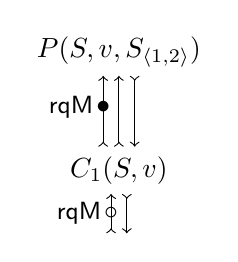
\begin{tikzpicture}
      \pic at (0, 0) {msipc1};
      \node[label={[label distance=-6pt]left:{\small {\sf rqM}}}] at (-0.2, -0.7) {$\bullet$};
      \node[label={[label distance=-6pt]left:{\small {\sf rqM}}}] at (-0.1, -2.05) {$\circ$};
    \end{tikzpicture}
    \caption{$C_1$ requesting to the parent}
    \label{fig-motive-2-a}
  \end{subfigure}
  \begin{subfigure}[b]{0.36\columnwidth}
    \centering
    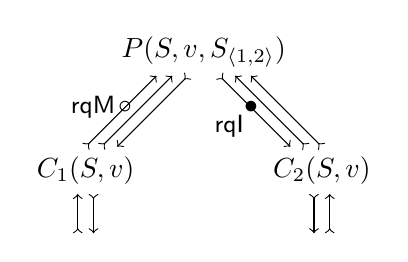
\begin{tikzpicture}
      \pic at (0, 0) {msi};
      \node[label={[label distance=-6pt]left:{\small {\sf rqM}}}] at (-1, -0.7) {$\circ$};
      \node[label={[label distance=-8pt]210:{\small {\sf rqI}}}] at (0.6, -0.7) {$\bullet$};
    \end{tikzpicture}
    \caption{$P$ making an invalidation request}
    \label{fig-motive-2-b}
  \end{subfigure}
  \begin{subfigure}[b]{0.30\columnwidth}
    \centering
    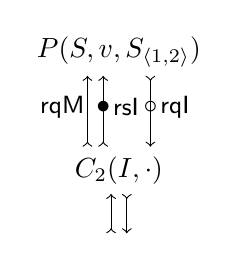
\begin{tikzpicture}
      \pic at (0, 0) {msipc2};
      \node[label={[label distance=-6pt]left:{\small {\sf rqM}}}] at (-0.4, -0.7) {$\blackdiamond$};
      \node[label={[label distance=-6pt]right:{\small {\sf rqI}}}] at (0.4, -0.7) {$\circ$};
      \node[label={[label distance=-6pt]right:{\small {\sf rsI}}}] at (-0.2, -0.7) {$\bullet$};
    \end{tikzpicture}
    \caption{$C_2$ responding to the parent}
    \label{fig-motive-2-c}
  \end{subfigure}
  \caption{Rule-execution cases in the simple MSI protocol}
  \vspace{-5pt}
  \label{fig-motive-2}
\end{figure}

All objects run concurrently, repeatedly executing \emph{rules} that define local state transitions.
In message-passing systems, a rule may take some messages from input channels, perform a state transition, and put messages in output channels.
A rule may also have a precondition, blocking use of that rule when the precondition does not hold.
\autoref{fig-motive-2} shows some example rule-execution cases depending on statuses of the objects.
\autoref{fig-motive-2-a} is the case where a child $C_1$ takes an external request ($\textsf{rqM}\circ$) to write data, but it does not have M status and thus forwards the request to the parent ($\textsf{rqM}\bullet$).
At this moment the child usually \emph{sets a lock} not to allow any further external requests for the value.
The following pseudocode describes the rule:
\begin{lstlisting}
Rule c1RqMToP :=
  assert !C1.locked();
  assert (C1.status != M);
  assert (C1.extRq.first == rqM);
  C1.extRq.deq();
  C1.rqToP.enq(rqM);
  C1.lock();
Endrule
\end{lstlisting}
The rule checks whether $C_1$ is not locked so it can handle $\textsf{rqM}\circ$, confirms it does not have a write permission, dequeues an external request from \slstinline{extRq}, sends a request to $P$ by using a channel \slstinline{rqToP}, and sets a lock.

As a next rule-execution step, $\textsf{rqM}\circ$ (previously outputted from \autoref{fig-motive-2-a}) is handled by the parent $P$, as shown in \autoref{fig-motive-2-b}.
It makes \emph{invalidation} requests ($\textsf{rqI}$) to the other children ($C_2$ is the only other child in this system) to change their statuses to I, since when a child has M the others should not be able to read/write the data.
After making invalidation requests, the parent also sets a lock to disallow requests from the children.

Now imagine a scenario where two children $C_1$ and $C_2$ requested $\textsf{rqM}$ to the parent (to obtain M) at the same time, and the parent decided to deal with the request from $C_1$ first.
Proper locking is indeed required here, since otherwise the parent will handle two $\textsf{rqM}$s simultaneously, which might lead to an incoherent state -- two M statuses in the system.
\autoref{fig-motive-2-c} presents this case, where an invalidation request was made to $C_2$ ($\textsf{rqI}\circ$) and even before this, $C_2$ requested $\textsf{rqM}\blackdiamond$ to the parent.
In order to handle all the requests correctly, we should carefully consider some corner cases:
\begin{itemize}[leftmargin=*]
\item Since $C_2$ requested $\textsf{rqM}\blackdiamond$, it is locked when the $\textsf{rqI}\circ$ message arrives. It should still be able to handle this invalidation request even if it is locked. We see that \emph{locking should be fine-grained enough to distinguish message kinds} while handling a request.
\item Due to the existence of $\textsf{rqM}\blackdiamond$, if we had a single channel from a child to a parent, a deadlock would occur. $P$ cannot take $\textsf{rqM}\blackdiamond$ since it was locked after making an invalidation request. It cannot take $\textsf{rsI}\bullet$ as well since the response is not the first one of the ordered channel. This case shows the necessity of having multiple channels between a child and a parent.
\end{itemize}

A so-called three-channel system has been widely used and regarded as a good choice to make the design correct and live~\cite{Murali:2015,thesis:Murali:2016}.
While there are other possible correct topology and network settings, the cases shown in \autoref{fig-motive-2} at least demonstrate that it is nontrivial to construct one of them.

If proper topology and locking are crucial for designing a correct protocol, can we craft a domain-specific language where only conformant protocols are expressible?
That is exactly what we plan to reflect in \hemiola{}, where, for instance, instead of the above pseudocode, rules are written more like the following one:
\begin{lstlisting}
Rule c1RqMToP :=
  using template RqToP;
  accepts rqM;
  assert (me.status != M);
  release rqM;
Endrule
\end{lstlisting}
Note that this pseudocode does not mention specific channels or locking at all.
Instead, it just says that the rule is for making a request to the parent (\slstinline{RqToP}), and it gives various associated assertions and actions, fitting slots associated with this kind of rule.

\hemiola{} provides \emph{rule templates} that employ proven-safe topologies and network structures and automatically set associated locks, so designers can design protocols without worrying about corner cases due to interleavings.

We further discovered that if a system is defined by using these rule templates, global invariants can be proven without explicit consideration of interference by concurrently executing memory accesses.
The key is the notion of \emph{serializability} coming originally from the database-transactions literature.

\subsection{Formal notion of serializability}

\subsubsection{Baseline: protocol transition systems}
\label{sec-trs}

\paragraph{Notations.}
Throughout this proposal, we will use several notations for lists (sequences) and finite maps.
A bold character (\eg{} $\listof{l}$) denotes a list.
$\listnil{}$, $(\listcons{h}{\listof{t}})$, $(\listapp{\listof{l_1}}{\listof{l_2}})$, $(\listsub{\listof{l_1}}{\listof{l_2}})$, and
$(\listdisj{\listof{l_1}}{\listof{l_2}})$ denote nil, cons, append, subtraction, and disjointness of lists, respectively.
$\listconcat{\listof{l}}$ flattens the list of lists $\listof{l}$ with repeated concatenation.
$\sizeof{\listof{l}}$ is the length of a list.
Regarding a list of key-value pairs as a finite map, we override notations for lists.
For example, $(\mapupds{M}{\listof{l}})$ updates multiple key-value pairs in a finite map $M$.
Moreover, we overload the same operation $(\mapupd{M}{k}{v})$ for a single update for simplicity.

\paragraph{Syntax.}

\begin{figure}[h]
  \centering\small
  \begin{tabular}{|c|c|}
    \hline
    \begin{math}
      \begin{array}{rl}
        \textrm{Index} & i \in \hidt{} \\
        \textrm{Value} & v \in \hvaluet{} \\
        \textrm{Message} & m ::= \tuple{i, v} \in \hmsgt{} \triangleq \hidt \ast \hvaluet \\
        \textrm{Object state} & o \in \hostt{} \\
        \textrm{Rule precondition} & p \in
        \hprect \triangleq \hostt \to \listtof{\hidmt} \to \propt \\
        \textrm{Rule transition} & t \in
        \htrst \triangleq \hostt \to \listtof{\hidmt} \to \hostt \ast \listtof{\hidmt} \\
      \end{array}
    \end{math} &
    \begin{math}
      \begin{array}{rl}
        \textrm{Rule} & r ::= \tuple{i, p, t} \\
        \textrm{Object} & O ::= \tuple{i, \listof{r}} \\
        \textrm{System} & S ::= \hsyss{\listof{O}}{i} \\
      \end{array}
    \end{math}\\
    \hline
  \end{tabular}
  \caption{Protocol transition system}
  \label{fig-trs-system}
\end{figure}

We first formally define protocol transition systems, which will be an underlying basis for the domain-specific language in \hemiola{}.
\autoref{fig-trs-system} explains what such systems are, in the style of automata theory.
Our definition is shallowly embedded in Coq, \eg{} precondition and transition definitions use native Coq function types.
A struct (a rule, an object, etc.)  sometimes has an \emph{index} to distinguish it from the other components.
We will use $\tuple{\cdot}$ to denote a struct and use a name to access a field value.
In our implementation, an index is a list of natural numbers, for easy hierarchical addressing.
A \emph{value} $v$ refers to a general set of values, principally those that can be stored at memory addresses.
A \emph{message} $m$ consists of a message id (effectively from an enumeration of message kinds) and value.

A system $S$ contains information about objects and channels.
It consists of objects (\listof{O}) and channel indices for internal messages (\hsysIn{i}), external inputs (\hsysRq{i}), and external outputs (\hsysRs{i}).
Each object (or channel) has its own unique index.
The definition is general in that any object can access any channel in the system, just by mentioning the channel index in a state transition.
It is necessary to distinguish between internal and external channels, in order to define external behaviors of the system.
An object $O$ contains its object index (unique within a system) and rules (\listof{r}) that make local state transitions within the object.

A rule $r$ consists of its rule index (unique within an object), a precondition ($p$), and a transition function ($t$).
A precondition takes two arguments, a current object state and a list of (channel index, message) pairs as input messages, and decides whether the rule can be executed or not.
A transition function takes the same arguments but returns the next object state and a list of (channel index, message) pairs as output messages.

\begin{figure*}[t]
  \centering
  \begin{tabular}{|c|}
    \hline
    \begin{math}
      \begin{array}{c}
        \inference[StepSilent:]{}{\semstep{S}{s}{\lblEmpty{}}{s}} \\
        \mbox{}\vspace{-5pt} \\ %% padding
        \inference[StepIns:]{\listof{m} \neq \listnil
          & \listof{\idxOf{m}} \subseteq \hsysRqA{S}
          & \nodup{\listof{\idxOf{m}}}}{\semstep{S}
          {\hst{\listof{o}}{M}}
          {\lblIns{\listof{m}}}
          {\hst{\listof{o}}{\enqMsgs{M}{\listof{m}}}}} \\
        \mbox{}\vspace{-5pt} \\ %% padding
        \inference[StepOuts:]{\listof{m} \neq \listnil
          & \listof{\idxOf{m}} \subseteq \hsysRsA{S}
          & \nodup{\listof{\idxOf{m}}}}{\semstep{S}
          {\hst{\listof{o}}{M}}
          {\lblOuts{\listof{m}}}
          {\hst{\listof{o}}{\deqMsgs{M}{\listof{m}}}}} \\
        \mbox{}\vspace{-5pt} \\ %% padding
        \inference[StepInt:]{S = \hsyss{\listof{O}}{i}
          & O \in S.\listof{O}
          & r \in O.\listof{r} \\
          \midxIns{m} \subseteq \hsysInA{S} \cup \hsysRqA{S}
          & \nodup{\midxIns{m}} \\
          \listof{o}\ \idxOf{O} = o_0
          & r.p\ o_0\ \msgIns{m}
          & r.t\ o_0\ \msgIns{m} = (o_1, \msgOuts{m}) \\
          \midxOuts{m} \subseteq \hsysInA{S} \cup \hsysRsA{S}
          & \nodup{\midxOuts{m}}
          & \disj{\midxIns{m}}{\midxOuts{m}}}{\semstep{S}
          {\hst{\listof{o}}{M}}
          {\lblInt{\idxOf{O}}{\idxOf{r}}{\msgIns{m}}{\msgOuts{m}}}
          {\hstm{\mapupd{\listof{o}}{\idxOf{O}}{o_1}}{\enqMsgs{\deqMsgs{M}{\msgIns{m}}}{\msgOuts{m}}}}} \\
        \mbox{}\vspace{-5pt} \\ %% padding
      \end{array}
    \end{math}\\
    \hline
    \begin{math}
      \begin{array}{ccc}
        \mbox{}\vspace{-5pt} \\ %% padding
        \inference[StepsNil:]{}{\semsteps{S}{s}{\listnil{}}{s}} &
        \inference[StepsCons:]{\semsteps{S}{s_0}{\listof{l}}{s_1}
          & \semstep{S}{s_1}{l_1}{s_2}}{\semsteps{S}{s_0}{\listcons{l_1}{\listof{l}}}{s_2}} &
        \inference[Behavior:]{\semsteps{S}{\sysInit{S}}{\listof{l}}{s}}{\sembeh{S}{\behOf{\listof{l}}}} \\
        \mbox{}\vspace{-5pt} \\ %% padding
      \end{array}
    \end{math}\\
    \hline
  \end{tabular}
  \caption{Semantics of protocol transition systems}
  \vspace{-10pt}
  \label{fig-trs-semantics}
\end{figure*}

\paragraph{Semantics.}
\autoref{fig-trs-semantics} describes the semantics of protocol transition systems.
A state transition (step) happens by a rule that takes input messages and generates output messages.
The semantics for a step is presented as a judgment $\semstep{S}{s_0}{l}{s_1}$, where $S$ is the system to execute, $s_0$ is a prestate, $s_1$ is a poststate, and $l$ is a label generated by the state transition.
The state of a system (in domain $\hsyst{}$) is a pair, consisting of object states and message states.
Object states are represented in finite maps from object indices to object states, and message states are represented in finite maps from channel indices to queues of messages.

Rule [StepSilent] represents the case where no state transition happens in the current step; an empty label (\lblEmpty{}) is generated in this case.
A system may accept input messages from the external world; [StepIns] describes this case, where the external input messages (\listof{m}) should not be empty, channels of the messages are valid, and none of them share the same channel ($\nodup{\listof{\idxOf{m}}}$); an external inputs label $(\lblIns{\listof{m}})$ is generated in this case.
[StepOuts] describes the opposite case, for output messages being released to the external world.

Lastly, [StepInt] deals with a state transition by a rule ($r$) in an object ($O$).
It nondeterministically chooses an object and a rule in the object, checks that the precondition holds, and applies the transition to update the state of the system; an internal label ($\lblInt{\idxOf{O}}{\idxOf{r}}{\msgIns{m}}{\msgOuts{m}}$) is generated in this case, which records an object index, a rule index, input messages, and output messages.

Note that the semantics is based on ordered channels, so messages are \emph{enqueued} and \emph{dequeued} in each state-transition case.
We use notations $\enqMsgs{M}{\listof{m}}$ and $\deqMsgs{M}{\listof{m}}$ for such operations, and especially when messages are dequeued we implicitly assume that each element in $\listof{m}$ is at the front of its queue.
It is also required that any state transition does not both dequeue and enqueue an element from the same queue; $\disj{\midxIns{m}}{\midxOuts{m}}$ in [StepInt] exactly describes this condition.

The step semantics is naturally lifted to one for multiple steps, presented as a judgment $\semsteps{S}{s_0}{\listof{l}}{s_1}$, where $S$, $s_0$, and $s_1$ are similar to ones in the step semantics, and $\listof{l}$ is a sequence of labels generated by executions of the steps.
[StepsNil] serves the case where no state transitions happen at all.
[StepsCons] is a natural inductive constructor that combines previous steps and a new one.
Note that the latest label is added to the head, thus the last label in the sequence is the oldest one.
(We found this convention convenient in Coq for usual reasons of functional-programming naturalness, and we stick with it in the paper version of the formalism to avoid transcription errors.)

We will sometimes call a sequence of labels a \emph{history}.
We say that a state $s$ is \emph{reachable} iff there is a history $\listof{l}$ such that $\semsteps{S}{\sysInit{S}}{\listof{l}}{s}$ holds.
We use a simpler notation $\semrch{S}{s}$ for reachable states.
We also apply the symmetrical notion that a history $\listof{l}$ is \emph{legal} iff there is a state $s$ such that $\semsteps{S}{\sysInit{S}}{\listof{l}}{s}$ holds.
We write $\semleg{S}{\listof{l}}$ to assert that a history is legal.

\paragraph{Behaviors and correctness.}
A system $S$ has a behavior $\behOf{\listof{l}}$ if there exists an execution of steps that generates $\listof{l}$, starting with the initial state of $S$ ([Behavior]).
Here the $\behOf{\cdot}$ operation filters out silent ($l_\epsilon$) and internal ($l_{\textrm{int}}$) labels so only the external parts remain.
We call such a sequence of labels a \emph{trace}.
Finally we define a notion of correctness in \hemiola{}.

\begin{definition}[Trace Refinement]
  A system $I$ (``implementation'') is said to trace-refine another system $S$
  (``specification''), written as $\refines{I}{S}$, iff every trace of $I$ is
  also a trace of $S$:
  \begin{displaymath}
    \refines{I}{S} \triangleq \forall \listof{t}.\; \sembeh{I}{\listof{t}} \to \sembeh{S}{\listof{t}}.
  \end{displaymath}
\end{definition}

\subsubsection{Serializability in protocol transition systems}

Serializability~\cite{sz1,sz2} is a celebrated notion of concurrency correctness that originated with databases and distributed systems.
While each transaction in a system affects multiple values, serializability guarantees that concurrent execution of such transactions is correct in that the effect (state change) is the same as if the transactions were executed serially, \ie{} atomically in some order with no interleaving.
The protocol transition system described in \autoref{sec-trs} follows standard ideas of message-passing systems, thus it is natural to define and reason about serializability.

\begin{figure}[t]
  \centering
  \begin{tabular}{|c|}
    \hline
    \begin{math}
      \arraycolsep=-2pt
      \begin{array}{c}
        \inference[AtomicStart:]{}{\atomicLong{\listof{\amsgi{m}}}{\listsingle{\lblInt{\idxOf{O}}{\idxOf{r}}{\listof{\amsgi{m}}}{\listof{\amsge{m}}}}}{\listof{\amsge{m}}}} \\
        \inference[AtomicCont:]{\atomic{\listof{\amsgi{m}}}{\listof{l}}{\listof{\amsge{m}}}
          & \msgIns{n} \neq \listnil
          & \msgIns{n} \subseteq \listof{\amsge{m}}}{\atomicLong{\listof{m_0}}{\listcons{\lblInt{\idxOf{O}}{\idxOf{r}}{\msgIns{n}}{\msgOuts{n}}}{\listof{l}}}{(\listapp{\listsub{\listof{\amsge{m}}}{\msgIns{n}}}{\msgOuts{n}}})} \\
        \mbox{}\vspace{-5pt} %% padding
      \end{array}
    \end{math}\\
    \hline
    \begin{math}
      \begin{array}{cc}
        \begin{array}{c}
          \inference[TrsSilent:]{}{\trsn{S}{\listsingle{\lblEmpty{}}}} \\
          \inference[TrsIns:]{}{\trsn{S}{\listsingle{\lblIns{\listof{m}}}}} \\
          \inference[TrsOuts:]{}{\trsn{S}{\listsingle{\lblOuts{\listof{m}}}}} \\
          \mbox{}\vspace{-5pt} %% padding
        \end{array} &
        \begin{array}{l}
          \textrm{\footnotesize TrsAtomic:} \\
          \inference[]{\extatomic{S}{\listof{\amsgi{m}}}{\listof{l}}{\listof{\amsge{m}}}}{\trsn{S}{\listof{l}}}
        \end{array} \\
      \end{array}
    \end{math}\\
    \hline
  \end{tabular}
  \caption{Atomic histories and transactions}
  \vspace{-5pt}
  \label{fig-hemiola-trs}
\end{figure}

\paragraph{Atomic histories.}
In order to define serializability formally, we first provide basic definitions of atomic histories and transactions, in \autoref{fig-hemiola-trs}.
A history $h$ is \emph{atomic} iff it satisfies the predicate $(\atomic{\listof{\amsgi{m}}}{h}{\listof{\amsge{m}}})$ with \emph{starting messages} $\listof{\amsgi{m}}$ and \emph{live messages} $\listof{\amsge{m}}$.
[AtomicStart] initializes a history with an internal label for its first step.
[AtomicCont] inductively adds a label to an atomic history, where the input messages of the new label should be from live messages of the previous atomic history.

\begin{figure}[h]
  \centering
  \begin{tabular}{c}
    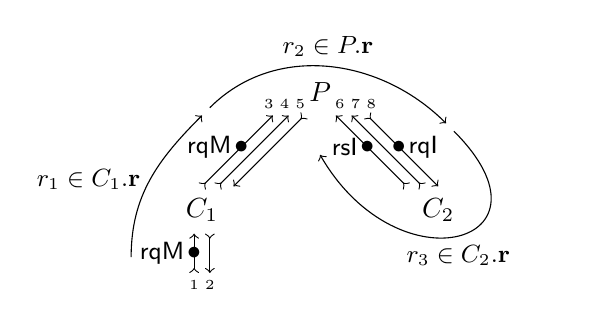
\begin{tikzpicture}
      \node at (0, 0) {$P$};
      \node at (-1.5, -1.5) {$C_1$};
      \node at (1.5, -1.5) {$C_2$};
      % between P and C_1
      \draw [<-<] (-0.6, -0.3) -- (-1.5, -1.2);
      \draw [<-<] (-0.4, -0.3) -- (-1.3, -1.2);
      \draw [>->] (-0.2, -0.3) -- (-1.1, -1.2);
      \node at (-0.65, -0.15) {\tiny $3$};
      \node at (-0.45, -0.15) {\tiny $4$};
      \node at (-0.25, -0.15) {\tiny $5$};
      \node[label={[label distance=-6pt]left:{\small {\sf rqM}}}] at (-1, -0.7) {$\bullet$};
      % between P and C_2
      \draw [>->] (0.6, -0.3) -- (1.5, -1.2);
      \draw [<-<] (0.4, -0.3) -- (1.3, -1.2);
      \draw [<-<] (0.2, -0.3) -- (1.1, -1.2);
      \node at (0.65, -0.15) {\tiny $8$};
      \node at (0.45, -0.15) {\tiny $7$};
      \node at (0.25, -0.15) {\tiny $6$};
      \node[label={[label distance=-6pt]left:{\small {\sf rsI}}}] at (0.6, -0.7) {$\bullet$};
      \node[label={[label distance=-6pt]right:{\small {\sf rqI}}}] at (1, -0.7) {$\bullet$};
      % C_1 external
      \draw [<-<] (-1.6, -1.8) -- (-1.6, -2.3);
      \draw [>->] (-1.4, -1.8) -- (-1.4, -2.3);
      \node at (-1.6, -2.45) {\tiny $1$};
      \node at (-1.4, -2.45) {\tiny $2$};
      \node[label={[label distance=-6pt]left:{\small {\sf rqM}}}] at (-1.6, -2.05) {$\bullet$};
      % C_2 external
      %% \draw [dotted] (1.6, -1.8) -- (1.6, -2.3);
      %% \draw [dotted] (1.4, -1.8) -- (1.4, -2.3);
      % Curves
      \draw [->] (-2.4, -2.1) to[out=90,in=-135] node[left] {\small $r_1 \in \hobjrules{C_1}$} (-1.5, -0.3);
      \draw [->] (-1.4, -0.2) to[out=45,in=135] node[above] {\small $r_2 \in \hobjrules{P}$} (1.6, -0.4);
      \draw [->] (1.7, -0.5) to[out=-45,in=-60,distance=2cm] node[below] {\small $r_3 \in \hobjrules{C_2}$} (0, -0.8);

    \end{tikzpicture}\\
    \hline
    \begin{math}
      \small
      \begin{array}{rl}
        h \triangleq & [\lblInt{\idxOf{C_1}}{\idxOf{r_1}}{\listsingle{(1, \textsf{rqM})}}{\listsingle{(3, \textsf{rqM})}};\\
        & \lblInt{\idxOf{P}}{\idxOf{r_2}}{\listsingle{(3, \textsf{rqM})}}{\listsingle{(8, \textsf{rqI})}};\\
        & \lblInt{\idxOf{C_2}}{\idxOf{r_3}}{\listsingle{(8, \textsf{rqI})}}{\listsingle{(6, \textsf{rsI})}}]\\
      \end{array}
    \end{math}
  \end{tabular}
  \caption{An example of an atomic history}
  \vspace{-5pt}
  \label{fig-ex-atomic-history}
\end{figure}

\autoref{fig-ex-atomic-history} presents an example of an atomic history.
$h$ is generated by executions of three rules, $r_1 \in \hobjrules{C_1}$, $r_2 \in \hobjrules{P}$, and $r_3 \in \hobjrules{C_2}$.
Rule $r_1$ takes an input message $\textsf{rqM}$ from the channel with index $1$, as a starting message of the history.
Rule $r_2$ takes $\textsf{rqM}$ from channel $3$, which held the output message from $r_1$.
Finally, $r_3$ takes $\textsf{rqI}$ from channel $8$, which is the output message from $r_2$.
Summing up all the rule executions, by the definition of an atomic history we get the predicate $\atomic{\listsingle{(1,\textsf{rqM})}}{h}{\listsingle{(6,\textsf{rsI})}}$.
This example shows that an atomic history intuitively captures a \emph{transaction flow} triggered by the starting messages.
Note that an atomic history does not need to be a completed transaction.
The history $h$ in the example is not completed, in the sense that the live message ($\textsf{rsI}$) is not a response to an external channel.

We call a history \emph{externally atomic} (denoted as \extatomic{S}{\listof{\amsgi{m}}}{\listof{l}}{\listof{\amsge{m}}}) if starting
messages are external requests ($\listof{\amsgi{m}} \subseteq \hsysRqA{S}$).
In other words, an externally atomic history records the way the system responded to some set of messages received from the outside world.

\paragraph{Transactions.}
Transactions are the next level of abstraction, defined by the final rules in \autoref{fig-hemiola-trs}.
A transaction is either a single silent label ([TrsSilent]), a single external inputs label ([TrsIns]), a single external outputs label ([TrsOuts]), or an externally atomic history ([TrsAtomic]).
In other words, the permitted atomic execution steps, in this transactional semantics, are arrival of new messages from the outside world, release of messages to the outside world, or uninterrupted execution of an atomic history.
We denote by $\trsn{S}{h}$ that $h$ is a transaction in $S$.

Note that an external-inputs label and an atomic history are regarded as separate transactions, thus the atomic history can start with inputs from multiple external-inputs labels.
This relaxed design choice is due to our eventual goal, trace refinement.
In order to prove trace refinement, we should preserve the \emph{order of external labels} while reasoning over histories.
In particular, we do not want a serialized history having a different trace from the original history.
A key soundness proof of \hemiola{} will reason with reorderings of internal steps and thus atomic histories, but we will leave external labels untouched, manifestly preserving trace orders.

\paragraph{Sequential histories and serializability.}
With a clear notion of transactions, we can easily define sequential histories and serializability.

\begin{definition}[Sequential Histories]
  A history $h$ is \emph{sequential} iff the history is a concatenation of
  transactions:
  \begin{displaymath}
    \hseq{S}{h} \triangleq \exists \listof{t}.\; (\forall t \in \listof{t}.\; \trsn{S}{t}) \wedge h = \listconcat{\listof{t}}.
  \end{displaymath}
  \label{def-seq}
\end{definition}

\begin{definition}[Serializability]\mbox{}\\
  \begin{enumerate}
  \item A legal history $h$ is \emph{serializable} in the system $S$ iff there
    exists a sequential history that reaches the same state:
    \begin{displaymath}
      \hsrzl{S}{h} \triangleq \forall s.\; \semsteps{S}{\sysInit{S}}{h}{s} \to \exists h_{\textrm{seq}}.\; \hseq{S}{h_{\textrm{seq}}} \wedge \semsteps{S}{\sysInit{S}}{h_{\textrm{seq}}}{s}.
    \end{displaymath}
  \item A system $S$ is \emph{serializable} iff every legal history is serializable:
    \begin{displaymath}
      \hsrz{S} \triangleq \forall h.\; \hsrzl{S}{h}.
    \end{displaymath}
  \end{enumerate}
  \label{def-sz}
\end{definition}

Note that we are reasoning only about serializability of sequences of rule executions, taking for granted that rules can be executed atomically.
Here we appeal to a tradition of hardware-description approaches that guarantee rule-level serializability for this kind of design~\cite{fesi,kami,Murali:2015,Dave:2005,Dave:2007}.

\section{Proposed Work}

\subsection{\hemiola{} DSL and automated proof of serializability}
\label{sec-hemiola-dsl}

We would like to develop a simple means that helps prove the correctness of various cache-coherence protocols that use certain families of networks and locking mechanisms.
In fact, our new characterization in \hemiola{} will just require that the system is defined on a template provided by the framework.
More particularly, \hemiola{} limits protocols primarily by dictating network topologies and locking disciplines and by forcing rules to be defined using \emph{rule templates} from the list of nine we have identified.

\subsubsection{Topology and network requirements}

In order to employ the serializability guarantee in \hemiola{}, the objects in a given system should form a tree topology.
Most cache-coherent memory subsystems follow this topology, where leaf nodes correspond to L1 caches, and the root corresponds to the main memory.
A child and its parent in the tree communicate using the three channels shown in \autoref{sec-example}, \eg{} whenever a child wants to send a request to the parent, it should use the upward-request channel.

\hemiola{} as a Coq library generates the topology and network channels automatically from instances of a simple inductive type.
For example, the following tree definition will generate topology and channels for four L1 caches, two L2 caches, the last-level cache (LLC), and the main memory:
\begin{displaymath}
  t : \textit{tree} \triangleq \small{\textsf{Node [Node [Node [Leaf; Leaf]; Node [Leaf; Leaf]]]}}.
\end{displaymath}

\subsubsection{Locking mechanism}
\label{sec-locking-mechanism}

We saw in \autoref{sec-example} how correctness requires a fine-grained locking mechanism for communication between a child and its parent.
For example, revisiting the issue described in \autoref{fig-motive-2-b}, a child should be able to handle an invalidation request from the parent even if it is locked while waiting for a response to its own request.
\hemiola{} supports a general locking mechanism that can deal with this situation.
Instead of looking at the type of a message (\eg{} invalidation), the framework provides \emph{more relaxed} locking, just by looking at whether the message is from the parent or one of its children.
This relaxed locking mechanism is still sufficient to prove serializability.

\tikzset{
  uprightedge/.pic = {
    \draw [>->] (0.2, 0.25) -- (0.5, 0.75);
  },
}
\begin{figure}[h]
  \centering
  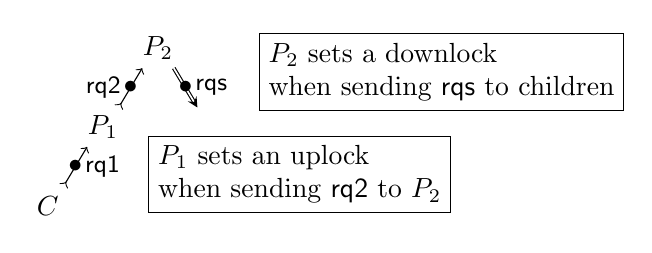
\begin{tikzpicture}
    \node at (0, 0) {$C$};
    \pic at (0, 0) {uprightedge};
    \node[label={[label distance=-6pt]right:{\small {\sf rq1}}}] at (0.35, 0.5) {$\bullet$};
    \node at (0.7, 1) {$P_1$};
    \pic at (0.7, 1) {uprightedge};
    \node[label={[label distance=-6pt]left:{\small {\sf rq2}}}] at (1.05, 1.5) {$\bullet$};
    \node at (1.4, 2) {$P_2$};

    \draw [>=stealth,double,->] (1.6, 1.75) -- (1.9, 1.25);
    \node[label={[label distance=-6pt]right:{\small {\sf rqs}}}] at (1.75, 1.5) {$\bullet$};

    \node[draw,align=left] at (3.2, 0.4) {$P_1$ sets an uplock\\ when sending $\textsf{rq2}$ to $P_2$};
    \node[draw,align=left] at (5.0, 1.7) {$P_2$ sets a downlock\\ when sending $\textsf{rqs}$ to children};
  \end{tikzpicture}
  \caption{Locking mechanism in Hemiola}
  \label{fig-locking}
\end{figure}

In particular, \hemiola{} provides two kinds of locks: \emph{uplocks and downlocks}.
We say an object is uplocked (or downlocked) when it holds an uplock (or downlock), respectively.
\autoref{fig-locking} depicts the locking mechanism in \hemiola{}.
An uplock is set when an object makes an upward request to its parent ($P_1$ in the figure); it is released when the object gets a corresponding response from the parent.
The object cannot make any further upward requests while uplocked, but \emph{it can handle requests from the parent}.
On the contrary, a downlock is set when an object makes a downward request(s) to some of its children ($P_2$ in the figure); similarly it is released when the object gets corresponding response(s) from the child requestee(s).
The object cannot make any further downward requests while downlocked.

\subsubsection{Rule templates}

\newcommand{\rtname}[1]{{\small\sf\bf #1}}

\newcommand{\uled}{\ensuremath{\textsf{UL}}}
\newcommand{\dled}{\ensuremath{\textsf{DL}}}
\newcommand{\ulfree}{\ensuremath{\textsf{UL}_{\times}}}
\newcommand{\dlfree}{\ensuremath{\textsf{DL}_{\times}}}

\newcommand{\setul}{\ensuremath{\textsf{UL}\Uparrow}}
\newcommand{\setdl}{\ensuremath{\textsf{DL}\Uparrow}}
\newcommand{\relul}{\ensuremath{\textsf{UL}\Downarrow}}
\newcommand{\reldl}{\ensuremath{\textsf{DL}\Downarrow}}
\newcommand{\stsilent}{\ensuremath{\textsf{SLT}}}

\newcommand{\ppo}[3]{\ensuremath{\{#1\}#2\lbrack#3\rbrack}}
\newcommand*{\bfrac}[2]{\genfrac{}{}{0pt}{}{#1}{#2}}

On top of the topology/network requirements and the locking mechanism, \hemiola{} provides rule templates to ensure that objects communicate within the topology and locks are properly set.

\begin{figure}[t]
  \centering
  \begin{subfigure}[b]{0.3\columnwidth}
    \centering
    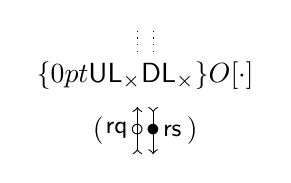
\begin{tikzpicture}
      \draw [dotted] (-0.1, 0.5) -- (-0.1, 0.8);
      \draw [dotted] (0.1, 0.5) -- (0.1, 0.8);
      \node at (0, 0.2) {$\ppo{\bfrac{\ulfree{}}{\dlfree{}}}{O}{\cdot}$};
      \draw [<-<] (-0.1, -0.2) -- (-0.1, -0.8);
      \draw [>->] (0.1, -0.2) -- (0.1, -0.8);
      \node[label={[label distance=-6pt]left:{\small {\sf rq}}}] at (-0.1, -0.5) {$\circ$};
      \node[label={[label distance=-6pt]right:{\small {\sf rs}}}] at (0.1, -0.5) {$\bullet$};
      \node at (0, -0.5) {$(\qquad\quad)$};
    \end{tikzpicture}
    \captionsetup{labelformat=empty}
    \caption{(a) immediate-down (\rtname{immd})}
  \end{subfigure}
  \begin{subfigure}[b]{0.3\columnwidth}
    \centering
    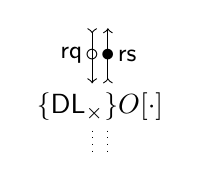
\begin{tikzpicture}
      \draw [<-<] (-0.1, 0.1) -- (-0.1, 0.8);
      \draw [>->] (0.1, 0.1) -- (0.1, 0.8);
      \node at (0, -0.2) {$\ppo{\dlfree{}}{O}{\cdot}$};
      \draw [dotted] (-0.1, -0.5) -- (-0.1, -0.8);
      \draw [dotted] (0.1, -0.5) -- (0.1, -0.8);
      \node[label={[label distance=-6pt]left:{\small {\sf rq}}}] at (-0.1, 0.45) {$\circ$};
      \node[label={[label distance=-6pt]right:{\small {\sf rs}}}] at (0.1, 0.45) {$\bullet$};
    \end{tikzpicture}
    \captionsetup{labelformat=empty}
    \caption{(b) immediate-up (\rtname{immu})}
  \end{subfigure}
  \begin{subfigure}[b]{0.3\columnwidth}
    \centering
    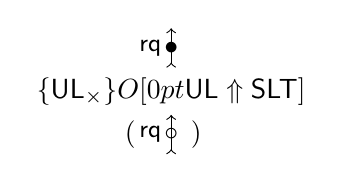
\begin{tikzpicture}
      \draw [>->] (0, 0.3) -- (0, 0.8);
      \node at (0, 0) {$\ppo{\ulfree{}}{O}{\bfrac{\setul{}}{\stsilent{}}}$};
      \draw [<-<] (0, -0.3) -- (0, -0.8);
      \node[label={[label distance=-6pt]left:{\small {\sf rq}}}] at (0, -0.55) {$\circ$};
      \node[label={[label distance=-6pt]left:{\small {\sf rq}}}] at (0, 0.55) {$\bullet$};
      \node at (-0.1, -0.55) {$(\qquad)$};
    \end{tikzpicture}
    \captionsetup{labelformat=empty}
    \caption{(c) request-up-up (\rtname{rquu})}
  \end{subfigure}
  \begin{subfigure}[b]{0.3\columnwidth}
    \centering
    \vspace{5pt}
    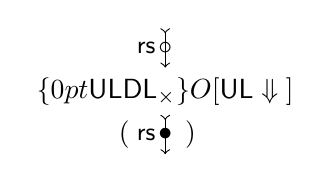
\begin{tikzpicture}
      \draw [<-<] (0, 0.3) -- (0, 0.8);
      \node at (0, 0) {$\ppo{\bfrac{\uled{}}{\dlfree{}}}{O}{\relul{}}$};
      \draw [>->] (0, -0.3) -- (0, -0.8);
      \node[label={[label distance=-6pt]left:{\small {\sf rs}}}] at (0, 0.55) {$\circ$};
      \node[label={[label distance=-6pt]left:{\small {\sf rs}}}] at (0, -0.55) {$\bullet$};
      \node at (-0.1, -0.55) {$(\qquad)$};
    \end{tikzpicture}
    \captionsetup{labelformat=empty}
    \caption{(d) response-down-down (\rtname{rsdd})}
  \end{subfigure}
  \begin{subfigure}[b]{0.3\columnwidth}
    \centering
    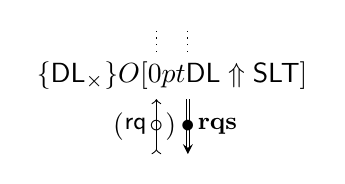
\begin{tikzpicture}
      \draw [dotted] (-0.2, 0.5) -- (-0.2, 0.8);
      \draw [dotted] (0.2, 0.5) -- (0.2, 0.8);
      \node at (0, 0.2) {$\ppo{\dlfree{}}{O}{\bfrac{\setdl{}}{\stsilent{}}}$};
      \draw [<-<] (-0.2, -0.1) -- (-0.2, -0.8);
      \draw [>=stealth,double,->] (0.2, -0.1) -- (0.2, -0.8);
      \node[label={[label distance=-6pt]left:{\small {\sf rq}}}] at (-0.2, -0.45) {$\circ$};
      \node[label={[label distance=-6pt]right:{\small {\sf {\bf rqs}}}}] at (0.2, -0.45) {$\bullet$};
      \node at (-0.35, -0.45) {$(\enspace\quad)$};
    \end{tikzpicture}
    \captionsetup{labelformat=empty}
    \caption{(e) request-up-down (\rtname{rqud})}
  \end{subfigure}
  \begin{subfigure}[b]{0.3\columnwidth}
    \centering
    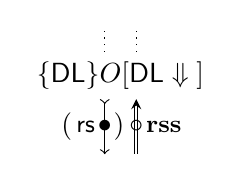
\begin{tikzpicture}
      \draw [dotted] (-0.2, 0.5) -- (-0.2, 0.8);
      \draw [dotted] (0.2, 0.5) -- (0.2, 0.8);
      \node at (0, 0.2) {$\ppo{\dled{}}{O}{\reldl{}}$};
      \draw [>->] (-0.2, -0.1) -- (-0.2, -0.8);
      \draw [>=stealth,double,<-] (0.2, -0.1) -- (0.2, -0.8);
      \node[label={[label distance=-6pt]left:{\small {\sf rs}}}] at (-0.2, -0.45) {$\bullet$};
      \node[label={[label distance=-6pt]right:{\small {\sf {\bf rss}}}}] at (0.2, -0.45) {$\circ$};
      \node at (-0.35, -0.45) {$(\enspace\quad)$};
    \end{tikzpicture}
    \captionsetup{labelformat=empty}
    \caption{(f) response-up-down (\rtname{rsud})}
  \end{subfigure}
  \begin{subfigure}[b]{0.3\columnwidth}
    \centering
    \vspace{5pt}
    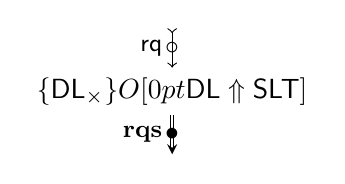
\begin{tikzpicture}
      \draw [<-<] (0, 0.3) -- (0, 0.8);
      \node at (0, 0) {$\ppo{\dlfree{}}{O}{\bfrac{\setdl{}}{\stsilent{}}}$};
      \draw [>=stealth,double,->] (0, -0.3) -- (0, -0.8);
      \node[label={[label distance=-6pt]left:{\small {\sf rq}}}] at (0, 0.55) {$\circ$};
      \node[label={[label distance=-6pt]left:{\small {\sf {\bf rqs}}}}] at (0, -0.55) {$\bullet$};
    \end{tikzpicture}
    \captionsetup{labelformat=empty}
    \caption{(g) request-down-down (\rtname{rqdd})}
  \end{subfigure}
  \begin{subfigure}[b]{0.3\columnwidth}
    \centering
    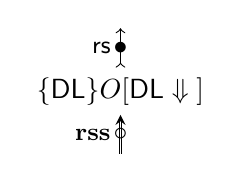
\begin{tikzpicture}
      \draw [>->] (0, 0.3) -- (0, 0.8);
      \node at (0, 0) {$\ppo{\dled{}}{O}{\reldl{}}$};
      \draw [>=stealth,double,<-] (0, -0.3) -- (0, -0.8);
      \node[label={[label distance=-6pt]left:{\small {\sf rs}}}] at (0, 0.55) {$\bullet$};
      \node[label={[label distance=-6pt]left:{\small {\sf {\bf rss}}}}] at (0, -0.55) {$\circ$};
    \end{tikzpicture}
    \captionsetup{labelformat=empty}
    \caption{(h) response-up-up (\rtname{rsuu})}
  \end{subfigure}
  \begin{subfigure}[b]{0.3\columnwidth}
    \centering
    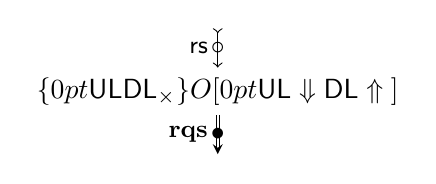
\begin{tikzpicture}
      \draw [<-<] (0, 0.3) -- (0, 0.8);
      \node at (0, 0) {$\ppo{\bfrac{\uled{}}{\dlfree{}}}{O}{\bfrac{\relul{}}{\setdl{}}}$};
      \draw [>=stealth,double,->] (0, -0.3) -- (0, -0.8);
      \node[label={[label distance=-6pt]left:{\small {\sf rs}}}] at (0, 0.55) {$\circ$};
      \node[label={[label distance=-6pt]left:{\small {\sf {\bf rqs}}}}] at (0, -0.55) {$\bullet$};
    \end{tikzpicture}
    \captionsetup{labelformat=empty}
    \caption{(i) resp-down-req-down (\rtname{rsrq})}
  \end{subfigure}
  \caption{Rule templates in Hemiola}
  \label{fig-rule-templates}
\end{figure}

\autoref{fig-rule-templates} presents the nine rule templates supported in \hemiola{}.
Each diagram has the form $\ppo{P}{O}{Q}$ and arrows with $\circ$ and $\bullet$.
It means that the rule template is for an object $O$, requires input messages ($\circ$) and a precondition $P$, performs a state transition $Q$, and generates output messages ($\bullet$).

$\uled$, $\dled$, $\ulfree$, and $\dlfree$ in a precondition indicate that the object is uplocked, downlocked, uplock-free, and downlock-free, respectively.
$\setul$, $\setdl$, $\relul$, and $\reldl$ in a state transition indicate setting an uplock, setting a downlock, releasing an uplock, and releasing a downlock, respectively.
$\stsilent{}$ annotates that the rule template forbids any state modification beside locking.

The rule templates are carefully designed to perform any practical transactions \emph{safely} with serializable behavior.
Considering an extreme case, in a cache-coherence protocol, if an L1 cache wants to obtain a write permission, all the other caches should be invalidated (changing each cache status to Invalid).
In order to perform such a transaction, it must be able to traverse all the other caches.
This transaction kind is one of the longest-running in cache-coherence protocols, and the rule templates are designed with proper locking ($\uled$ and $\dled$) and a state-change condition ($\stsilent$), not to create any incoherence while such a long transaction is interleaved with other transactions.

\subsubsection{Automated proof of serializability}

\newcommand{\ontree}[2]{\ensuremath{\textit{OnTree}\ #1\ #2}}
\newcommand{\goodrules}[2]{\ensuremath{\textit{GoodRules}\ #1\ #2}}

On top of the \hemiola{} DSL, we can now claim that the use of good topology and the rule templates automatically guarantees serializability:
\begin{theorem}[\hemiola{}'s serializability guarantee]
  \begin{displaymath}
    \forall S, t.\; \ontree{S}{t} \land \goodrules{S}{t} \to \hsrz{S},
  \end{displaymath}
  where $(\ontree{S}{t})$ requires that the system $S$ is well-defined on the topology/network $t$, and $(\goodrules{S}{t})$ requires that each rule in $S$ conforms to one of the rule templates.
  \label{thm-sz-guarantee}
\end{theorem}
While this theorem has been already proven, in order to achieve the completely automated proof, we need to prove \ontree{S}{t} and \goodrules{S}{t} automatically as well.
Each of these predicates is defined like a static checker that looks at the system definition, thus it is fair to say that automating these predicate proof is to build a verified validator.

%%%%%%%%%%%%%%%%%%%%%%%%%%%%%%%%%%%% TODO: FROM HERE
\subsection{Complete proofs of hierarchical noninclusive MSI and MESI protocols}

On top of the \hemiola{} framework, we would like to prove the correctness of hierarchical, noninclusive MSI and MESI protocols as case studies.
They use directories to keep track of child statuses and use noninclusive caches that do not require the parent cache to contain all lines existing in children.
We will also investigate how \hemiola{} helps implement and prove these protocols, by taking full advantage of \autoref{thm-sz-guarantee}.

\subsubsection{Design principles}
We start by summarizing the design principles we apply to both case studies.

\paragraph{Topology as a parameter.}

Each design is parameterized by a tree $t$ that decides the topology of the memory subsystem.
In other words, whenever we instantiate the tree parameter, we get a cache-coherence design and its correctness proof for free.
There are three different kinds of caches in this topology-parameterized protocol.
First of all, there are L1 caches (denoted as $L_1$) that correspond to leaf nodes in the tree.
Symmetrically, each uses the same set of rules.
The second kind is the last-level cache (LLC), which is the only one attached to the main memory, the root of the tree.
All the other caches between the L1 caches and the LLC are called intermediate caches (denoted as $L_i$), and they share a common set of rules as well.

\paragraph{Directory-based coherence.}

The protocol uses a well-known directory structure~\cite{Tang:1976} to ensure coherence.
In our designs, each node with children has its own directory structure to track their statuses.
The directory holds sound information about the status of each child \emph{subtree}.
For example, for a certain cache line, if an L1 cache $L_1$ has M status for the line, then all the ancestors (including the main memory) of $L_1$ have the directory status M pointing to the child subtree that contains $L_1$.

\paragraph{Voluntary evictions.}

The protocol allows voluntary evictions, \ie{} there are rules in each cache that can be executed even without being triggered by input messages, to evict a cache line.
This design itself is certainly not realistic, but it always has more behaviors than any design with specific eviction policies, thus in terms of correctness a refinement to a specific design is trivial.

\paragraph{Noninclusiveness.}

The protocol is noninclusive so the parent cache does not have to contain all the lines that children have, and back invalidations are not required to evict a line.
In inclusive caches, in order to maintain the inclusion policy, it is required to invalidate each cache line of a child recursively before evicting the parent's line, which adds overhead.
On the other hand, noninclusive caches do not need such a process, but it may take more time to read a clean line value, since the absence of a line in higher-level caches does not imply absence in lower-level caches, so we might have to search the lower-level caches.

\paragraph{Design and proof per-line.}

The protocol is defined just for a single cache line first, then naturally extended to all cache lines using a protocol compiler that will be introduced in \autoref{sec-synthesis}.
This approach is reasonable in terms of correctness, since a transaction does not affect coherence for lines other than its own.
Consider the ``duplicated'' protocol first, where each cache line, its status, a directory entry, communication channels, and a lock holder are all duplicated per-line.
It is infeasible to extend the protocol literally in this way, since we cannot require physically distinct channels and lock holders for all cache lines.
The protocol compiler restricts the resources (\eg{} channels, lock holders, etc.) to make the implementation hardware-synthesizable.

\subsubsection{The protocols: MSI and MESI}
\label{sec-protocols}

\newcommand{\mesi}{\ensuremath{\textsf{MESI}}}
\newcommand{\msi}{\ensuremath{\textsf{MSI}}}
\newcommand{\stM}{\ensuremath{\textsf{M}}}
\newcommand{\stE}{\ensuremath{\textsf{E}}}
\newcommand{\stS}{\ensuremath{\textsf{S}}}
\newcommand{\stI}{\ensuremath{\textsf{I}}}
\newcommand{\dir}[2]{\ensuremath{#1_{\tuple{#2}}}}

The MSI protocol is known as a base cache-coherence protocol that can be optimized to more sophisticated protocols like MESI, MOSI, etc.
Even though it is a base protocol, there are a lot of nontrivial cases that require deep understanding of the protocol itself and the nature of distributed protocols, especially in hierarchical protocols.
The MESI protocol~\cite{Papamarcos:1984} applies further optimizations to the MSI protocol, by adding a status called Exclusive-Unmodified.
As the name of the status says, if a cache line has \stE{} status, then the line is exclusive to the cache but also clean.

\subsubsection{Correctness proofs of the protocols}

The correctness proofs of the MSI and MESI protocols claim that the both implementations refine to a single-line memory as a spec.
Most of the time, a refinement proof requires two steps: 1) to prove \emph{invariants} of the implementation that help relating it to the spec and 2) to define and prove a \emph{simulation} relation between an implementation and the spec that directly implies a refinement.
We would like to demonstrate \hemiola{} helps proving necessary invariants for the correctness proofs.

\paragraph{Logical status of an object.}
The MSI protocol largely has three invariants, where each invariant corresponds to a desired property of one status -- \stM{}, \stS{}, and \stI{}.
For instance, we want to claim that whenever a cache has \stM{} status, all the other objects have \stI{} status.
Unfortunately, this invariant is not true, since there might be another cache that has not handled an invalidation response yet, thus retaining a valid status.

In order to deal with this subtlety, we introduce a notion called \emph{logical status} to obtain an abstract status of each object.
In the above example, even if the cache has not handled the invalidation response yet, the logical status is \stI{}.
Logical statuses are defined formally as follows:
\begin{itemize}[leftmargin=*]
\item An object has logical status \stM{} if the object has \stM{} and there is no invalidation response to the object.
\item It has logical status \stS{} if either 1) the object has \stS{} and there is no invalidation response to the object or 2) there is a response \slstinline{rsS} to the object.
\item It has logical status \stI{} if either 1) the object has \stI{} and there is no \slstinline{rsM} or \slstinline{rsS} to the object or 2) there is an invalidation response \slstinline{rsI} to the object.
\end{itemize}
Note that the logical status of an object is \emph{not} \stM{} when there is a response \slstinline{rsM} to the object, since the response could imply an ongoing invalidation process.

We should extend the notion of logical status for the MESI protocol, declaring that an object in MESI is \stE{} if either 1) the object has \stE{} and there is no invalidation response to the object or 2) there is a response \slstinline{rsE} to the object.

\paragraph{Invariants.}
Using the logical status of each object, we can state the desired invariant for each status:
\begin{itemize}[leftmargin=*]
\item The \emph{exclusiveness} invariant claims an expected property regarding \stM{} (or \stE{}) status. It says that whenever a cache (or the main memory) has logical status \stM{} (or \stE{}), then all the other caches are in logical \stI{} status.
\item The \emph{sharing} invariant claims that all objects in logical \stS{} status have the same value.
\item The \emph{invalidness} invariant claims that a certain set of objects are all in logical \stI{} status. Such a set may refer to the objects inside (or outside) a subtree of the system, determined by looking at the directory status or the ownership bit. For example, if an object $O$ has an ownership bit true, then all the objects outside $O$ have logical \stI{} status.
\item The invariant for \stE{} claims that if an object takes an invalidation request without writeback from a child, and the directory status pointing to the child is \stE{}, then the object has a coherent value.
\end{itemize}

\paragraph{Invariant proofs using predicate messages.}

\newcommand{\subtree}[1]{\ensuremath{\textrm{tr}(#1)}}
\newcommand{\subtreec}[1]{\ensuremath{\textrm{tr}^{-1}(#1)}}
\newcommand{\objsinv}[1]{\ensuremath{\textsf{Invalid}(#1)}}

While proving the sharing invariant is easy, it is nontrivial to prove the exclusiveness invariant and the invalidness invariant.

\begin{figure}[h]
  \centering
  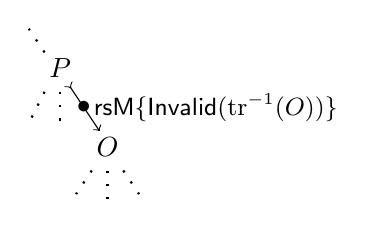
\begin{tikzpicture}
    \node at (0, 0) {$O$};
    \node at (-0.6, 1) {$P$};
    \draw [>->] (-0.5, 0.8) -- (-0.1, 0.2);
    \node[label={[label distance=-6pt]right:{\small $\textsf{rsM}\{\objsinv{\subtreec{O}}\}$}}] at (-0.3, 0.5) {$\bullet$};
    %% tr(O)
    \draw [thick,loosely dotted] (-0.2, -0.3) -- (-0.4, -0.6);
    \draw [thick,loosely dotted] (0, -0.3) -- (0, -0.7);
    \draw [thick,loosely dotted] (0.2, -0.3) -- (0.4, -0.6);
    %% tr-1(P)
    \draw [thick,loosely dotted] (-0.8, 0.7) -- (-1, 0.3);
    \draw [thick,loosely dotted] (-0.6, 0.7) -- (-0.6, 0.3);
    \draw [thick,loosely dotted] (-0.8, 1.2) -- (-1, 1.5);
  \end{tikzpicture}
  \caption{Predicate messages over \slstinline{rsM}}
  \label{fig-predicate-msg}
\end{figure}

The common underlying difficulty comes from stating invariants for certain types of messages.
For instance, \autoref{fig-predicate-msg} depicts what the desired invariant is when a message with the ID \slstinline{rsM} exists in the system.
Defining $\subtree{O}$ ($\subtreec{O}$) as a set of objects inside (outside) the subtree rooted at $O$, the desired invariant is that each object in $\subtreec{O}$ is in logically invalid state, denoted as $\objsinv{\subtreec{O}}$.
This invariant is indeed required at the moment when an L1 cache takes \slstinline{rsM} and changes its status to \stM{}.

We call this invariant over a specific message a \emph{predicate message}, since it is like a message carrying a predicate over the target system.
How could we prove the correctness of predicate messages?
A naive but typical approach is to strengthen the invariant repeatedly by manually considering possible states.
In the case of \slstinline{rsM}:
\begin{itemize}[leftmargin=*]
\item We should strengthen the invariant by claiming that each object in $\subtreec{O}$ cannot take \slstinline{rsS} as well; if there is an object that can take it, then its state becomes \stS{}, which violates the invariant.
\item Following the above case, we also should claim that an object in $\subtreec{O}$ cannot take \slstinline{downRsS}, otherwise it may take the message and release \slstinline{rsS}, which violates the invariant.
\item $\cdots$ we should repeat this process until the invariant is provable by induction, which checks each state transition by a rule.
\end{itemize}
Such a process represents a typical burden in stating and proving an invariant, especially in distributed systems.

Thanks to \hemiola{}'s serializability support, we need not strengthen the invariant at all.
Instead, we can employ \emph{atomic invariants}, restricting the proof to the predicates for live messages in a current atomic history.
Revisiting the case of \slstinline{rsM}, in the middle of an atomic history, \slstinline{rsM} is the only live message.
Now if we state the atomic invariant that provides a predicate for each live message, we do not need to worry about whether the predicates for the other live messages still hold when making a state transition with \slstinline{rsM}.

\paragraph{Refinement proofs.}

%% We just need minimum spacing to detach `Coh` and `Spec` from the left parenthesis `(`
\newcommand{\implcoh}[3]{\ensuremath{\textit{Coh}\,(#1, #2, #3)}}
\newcommand{\speccoh}[1]{\ensuremath{\textit{Spec}\,(v)}}

Once equipped with sufficient invariants, it is straightforward to prove the refinement between the implementation and the spec.
The only work is to define a correct simulation that relates all the coherent values in the implementation and the single value in the spec.
The coherent values are collected by looking at the logical status of each object; if the logical status is not \stI{} then values either in the object or in some messages (\eg{} \slstinline{rsS}) are coherent.

Denoting by $\implcoh{s}{o}{v}$ that an object state in a system state $s$ contains a coherent value $v$, the simulation can be stated as follows for the MSI protocol:
\begin{theorem}[Correctness of the MSI protocol]
  The following simulation relation holds between the implementation system state $s^I$ and the spec system state $s^S$.
  \begin{displaymath}
    s^I \sim s^S \triangleq \exists v.\; \forall o.\; \implcoh{s^I}{o}{v} \wedge s^S = \speccoh{v}.
  \end{displaymath}
  where $\speccoh{v}$ represents a single-value state for the spec.
\end{theorem}
The simulation relation for the MESI protocol is just the same as the one for the MSI protocol, while the coherence predicate $\implcoh{s^I}{o}{v}$ is extended slightly to cover objects with \stE{} status and messages with ID \slstinline{rsE}.

\subsection{Protocol compiler to synthesize \hemiola{} protocols}
\label{sec-synthesis}

As mentioned in \autoref{sec-protocols}, we have dealt with cache-coherence protocols for a single line, where the specification has a single line as well.
In order to build a hardware-synthesizable multiline implementation, we plan to develop a compiler that takes a single-line \hemiola{} protocol as a source program and generates a multiline implementation described in Kami~\cite{kami}.
Kami is a hardware formal-verification framework, where its own HDL and proof tools are defined in Coq, allowing users to design, specify, verify, and synthesize their hardware components.

The protocol transition system and the rule templates given in the \hemiola{} DSL match well rule-based HDLs like Kami; a rule in \hemiola{} naturally maps to an equivalent rule in Kami, which describes atomic state transitions in hardware modules.
Instead of directly compiling \hemiola{} protocols to a register-transfer language (RTL), we chose to build a compiler from \hemiola{} to Kami as a first step toward using the protocols and their correctness proofs within larger Kami proofs including processors -- though our experiments here do not include those composition proofs.
Since Kami already has a hardware-synthesis toolchain, we can just compile a \hemiola{} program to Kami and use the toolchain to run it on FPGAs.

\subsubsection{Compilation of a \hemiola{} protocol}
\label{sec-compiler}

\begin{figure}
  \centering
  \tikzstyle{arg} = [inner sep=1pt]
  \tikzstyle{component} = [rectangle, draw=black, inner sep=5pt, outer sep=2pt]
  \tikzstyle{libcomp} = [rectangle, draw=black, inner sep=3pt, outer sep=1pt, minimum width=2cm]
  \tikzstyle{arrow}=[-{stealth}]
  \tikzstyle{dataflow}=[-{latex}]
  \begin{tikzpicture}
    \node[arg] (hemiolaSource) at (0, 1.2) {\small\sf{(Single-line) \hemiola{} protocol}};
    \node[component] (compiler) at (0, 0) {\small\sf{Protocol Compiler}};
    \node[arg, fill=white] (kamiTarget) at (0, -1.2) {\small\sf{(Multiline) Kami implementation}};
    \node[anchor=east, arg] (extComp) at (-2, 0.4) {\scriptsize\sf{Custom data structure reifier/compiler}};
    \node[anchor=east, arg] (infoEnc) at (-2, 0) {\scriptsize\sf{Tag/Information encoder/decoder}};
    \node[anchor=east, arg] (cacheConfig) at (-2, -0.4) {\scriptsize\sf{Cache/MSHR configuration}};

    \node[anchor=west,
      rectangle, draw=black,
      minimum width=2.2cm,
      minimum height=1.5cm] (lib) at (2.5, 0) {};
    \node[above right] at (lib.north west) {\scriptsize\sf{Prebuilt Kami library}};
    \node[anchor=west, libcomp] (bitvector) at (2.6, 0.5) {\scriptsize\tt{Bitvector}};
    \node[anchor=west, libcomp] (cache) at (2.6, 0) {\scriptsize\tt{Cache}};
    \node[anchor=west, libcomp] (mshrs) at (2.6, -0.5) {\scriptsize\tt{MSHRs}};

    \draw [dataflow] (hemiolaSource) to
    node[left, inner sep=1pt] (reifyArrow) {}
    node[right] {\scriptsize\sf\it{after reification}} (compiler);
    \draw [dataflow] (compiler) to (kamiTarget);
    \draw [arrow] (extComp) to[out=0,in=180] (reifyArrow);
    \draw [arrow] (extComp) to[out=0,in=180] (compiler);
    \draw [arrow] (infoEnc) to (compiler);
    \draw [arrow] (cacheConfig) to[out=0,in=180] (compiler);
    \draw [arrow] (lib) to[out=180,in=0] (compiler);

    \node[anchor=west, arg] (bsvTarget) at (0.5, -1.7) {\small\sf{Bluespec implementation}};
    \node[anchor=west, arg] (fpga) at (2.7, -2.2) {\small\sf{Circuit on FPGA}};

    \draw [dataflow] (kamiTarget) to[out=270,in=180,outer sep=3pt] node[left] {\scriptsize\sf\it{Kami-to-Bluespec transliteration}} (bsvTarget);
    \draw [dataflow] (bsvTarget) to[out=270,in=180,outer sep=3pt] node[left] {\scriptsize\sf\it{Bluespec synthesis}} (fpga);

    \begin{pgfonlayer}{procomp}
      \node[anchor=west, text={rgb:black,3;white,1}, arg] at (-6.5, -1) {\scriptsize\sf\it{compilation}};
      \draw[dashed] (-6.5, -1.2) -- (5.5, -1.2);
      \node[anchor=west, text={rgb:black,3;white,1}, arg] at (-6.5, -1.4) {\scriptsize\sf\it{synthesis}};
    \end{pgfonlayer}
  \end{tikzpicture}
  \caption{Compilation and Synthesis of \hemiola{} protocols}
  \label{fig-compiler}
\end{figure}

\autoref{fig-compiler} depicts a compilation/synthesis flow from a given \hemiola{} protocol to an FPGA-ready circuit.
A source program of the protocol compiler is a single-line protocol described in \hemiola{} with the rule templates.

\paragraph{Preprocessing: reification.}

Before feeding a \hemiola{} source program to the compiler, a preprocessing step is required, which is to reify the program into an AST we can hand off to the compiler.
\hemiola{} supports automated, correct-by-construction reification driven by a series of tactics in Coq.
For instance, the rule-reification tactic (\slstinline{reify_rule}) reifies a \hemiola{} rule to the corresponding rule AST, where \slstinline{HRule} is a Coq \slstinline{Record} containing the AST and its correctness, \ie{} denotation of the AST matches the denotation of the original rule:
\begin{lstlisting}[numbers=none, frame=none, xleftmargin=10pt]
Definition hl1GetMImmE: HRule l1GetMImmE := ltac:(reify_rule).
\end{lstlisting}

\paragraph{Compiling asynchronous line accesses.}

One of the biggest differences between a source \hemiola{} protocol and the target Kami code is that the target accesses multiple lines \emph{asynchronously}.
In the source protocol, a single line can be read (or written) \emph{immediately} by directly accessing a value, whereas in the target the value is accessed asynchronously by making a read (or write) request with a certain line address to a cache and by handling the response.

In order to optimize asynchronous line accesses, we plan to make the protocol compiler transform a \hemiola{} rule into multiple Kami rules, each of which takes part of the source-rule execution.
Furthermore, we would like to optimize such rules to be executed in a \emph{pipelined} way, so that a status read and a value write for different addresses are executed in parallel.
This optimization is nontrivial but ubiquitous in real cache controllers.

\paragraph{Prebuilt hardware components.}
The compiler uses prebuilt hardware components described in Kami.
One of them is a cache, whose interface includes making read/write requests and getting the responses.
The cache normally uses a BRAM (block RAM), which is defined as a primitive in Kami.
The Kami BRAM is later synthesized to a BRAM on an FPGA.
The cache module also manages \emph{victim lines} that should be evicted eventually.
Optimization opportunities remain in the cache itself, especially for noninclusive caches.
To improve space efficiency, we plan to implement NCID~\cite{Zhao:2010,Yan:2019} that already has been used in industry.

Another prebuilt component holds a finite number of MSHRs, whose abstract interface includes registering, updating, and releasing MSHRs with respect to their types (uplock or downlock) and locking addresses.
Recall that ideally (as a spec) MSHRs are assigned per-line, but the actual design can contain only a finite number of them.
The compiler takes several counts as configuration parameters to determine the sizes of caches (\eg{} \#lines, \#ways) and MSHRs (\eg{} \#uplocks, \#downlocks).

\paragraph{Compiling custom data structures.}
Since a \hemiola{} protocol may use its own custom data structure (\eg{} directory structure for the MESI protocol), the compiler requires a user to provide a reifier and a compiler for it.
This task is straightforward for the user, since both reification and compilation work at the level of expressions, not rules.
For instance, a field access \slstinline{dir.(dir_sharers)} for a Coq record \slstinline{dir} is reified to an expression AST node \slstinline{(HDirGetSh hdir)}, where \slstinline{hdir} is the reified directory structure, and compiled to \slstinline{cdir@."dir_sharers"} in Kami, which uses a field-access expression.

\subsubsection{Correctness of a cache and its controller}

As explained in \autoref{sec-compiler}, the protocol compiler takes a cache configuration as an argument, thus we can have several different implementations by providing different configurations.
Then what would be the specification for all possible implementations from a given source protocol?
The core idea comes from the fact that \emph{the coherence of each line is orthogonal to coherence of others}.
In this case, a single-line \hemiola{} protocol is naturally extended to a multiline one by using the notion of compositionality.
Compositionality claims that if two systems are index-disjoint (\ie{} objects and channel indices are disjoint) thus not communicating with each other, then refinement of the composed system is obtained for free just by composing the specs:
\begin{theorem}[Compositionality]
  \begin{displaymath}
    \forall I_1, I_2, S_1, S_2.\ \refines{I_1}{S_1} \land \refines{I_2}{S_2} \to
    \refines{I_1 \oplus I_2}{S_1 \oplus S_2},
  \end{displaymath}
  where $I_1 \oplus I_2$ implicitly assumes that the indices used in $I_1$ and $I_2$ are disjoint.
\end{theorem}

\hemiola{} additionally supports an \emph{index-extension} mechanism, which takes a system $S$ and a \emph{prefix index} $i$, generating a new system $S^{(i)}$ where every object or channel index in the system is extended by attaching $i$.
Note that an index in \hemiola{} is a list of numbers, so it is easy to extend an index just by concatenating another one.
\hemiola{} also provides a lemma that $S^{(i)}$ and $S^{(j)}$ are index-disjoint when $i \neq j$.

Composing these elements, we obtain a replication theorem that is used directly to convert a single-line cache-coherence protocol to an ideal multiline protocol:
\begin{theorem}[Replication]
  $\forall I, S.\ \refines{I}{S} \to \forall n.\ \refines{\bigoplus^{n}_{i=0} I^{(i)}}{\bigoplus^{n}_{i=0} S^{(i)}}$.
  \label{thm-replication}
\end{theorem}

The multiline protocol derived from the replication theorem is indeed ideal; it has line values, lock holders, and communication channels per cache line.
Thus the protocol can serve as a spec for all the multiline implementations generated by the protocol compiler, since they have limited resources, which implies that the behavior of the multiline protocol covers their behaviors.

\begin{figure}[h]
  \centering
  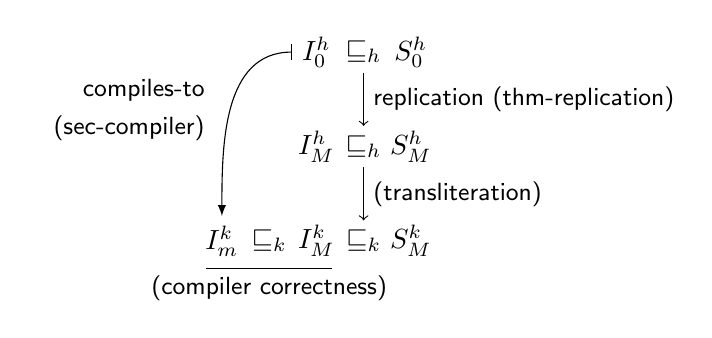
\begin{tikzpicture}
    \node (ih0) at (0, 0) {$I^{h}_{0}$};
    \node (rh0) at (0.6, 0) {$\sqsubseteq_{h}$};
    \node (sh0) at (1.2, 0) {$S^{h}_{0}$};

    \node (ihM) at (0, -1.2) {$I^{h}_{M}$};
    \node (rhM) at (0.6, -1.2) {$\sqsubseteq_{h}$};
    \node (shM) at (1.2, -1.2) {$S^{h}_{M}$};

    \node (ikm) at (-1.2, -2.4) {$I^{k}_{m}$};
    \node (rkm) at (-0.6, -2.4) {$\sqsubseteq_{k}$};
    \node (ikM) at (0, -2.4) {$I^{k}_{M}$};
    \node (rkM) at (0.6, -2.4) {$\sqsubseteq_{k}$};
    \node (skM) at (1.2, -2.4) {$S^{k}_{M}$};

    \draw (-1.4, -2.75) to (0.2, -2.75);
    \node (compCorrect) at (-0.6, -3.0) {\small\sf{(compiler correctness)}};

    \draw[|-{latex}] (ih0) to[out=180,in=90] node[left] {
      \small\sf\begin{tabular}{r}
      compiles-to\\
      (\autoref{sec-compiler})
      \end{tabular}} (ikm);
    \draw[->] (rh0) to node[right] {\small\sf{replication (\autoref{thm-replication})}} (rhM);
    \draw[->] (rhM) to node[right] {\small\sf{(transliteration)}} (rkM);
  \end{tikzpicture}
  \caption{A single-line protocol, a multiline spec, and multiline implementations}
  \label{fig-multiline-spec}
\end{figure}

\autoref{fig-multiline-spec} elaborates more on the role of the multiline specification.
For a given \hemiola{} single-line protocol ($I^{h}_{0}$), we can lift the refinement using the replication theorem to obtain a refinement for the multiline protocol ($I^{h}_{M}$).
Since both \hemiola{} and Kami are rule-based description languages, we expect it is straightforward to have an ideal multiline protocol in Kami ($I^{k}_{M}$) in the sense of simple transliteration, while preserving the refinement.
After all, the correctness of the protocol compiler must be the refinement from a target Kami implementation ($I^{k}_{m}$) to the multiline protocol.
Proving compiler correctness in this manner is on our list of valuable future work -- we would like to prove and describe the compiler correctness in the thesis, if time permits.

\section{Timeline and Milestones}

\begin{figure}[h]
  \renewcommand{\arraystretch}{1.25}
  \centering\small
  \begin{tabular}{r|l}
    \hline
    \multirow{3}{*}{Sep 2020} & \bf \hemiola{} DSL and the serializability proof \\
    & \quad Clean up the current DSL definitions and proof code \\
    & \quad Automate the rule-template checker \\
    \hline
    \multirow{2}{*}{Oct 2020} & \bf Complete proofs of the case-study protocols \\
    & \quad Clean up all the proofs \\
    \hline
    \multirow{4}{*}{Sep -- Dec 2020} & \bf Protocol compiler to synthesize \hemiola{} protocols \\
    & \quad Design the cache interface + Implement NCID \\
    & \quad Design and implement the cache-controller pipeline \\
    & \quad Evaluate the protocol implementation \\
    \hline
    Oct 2020 -- Jan 2021 & \bf Write thesis \\
    Dec 11, 2020 & \quad Thesis title submission deadline \\
    Jan 8, 2021 & \quad PhD thesis submission deadline \\
    Nov -- Dec 2020 & Prepare presentation for thesis defense \\
    Dec 2020 & \bf Thesis defense \\
    \hline
  \end{tabular}
\end{figure}


